\section{EEG en búsqueda visual}
\label{sec:eeg_modelo_damian}

% Presentar el EEG como herramienta para estudiar la actividad neural
% durante búsqueda visual. Presentar el pipeline de análisis de Damián:
% deconvolución lineal (TRF), regularización Ridge, y los predictores
% del modelo base.

El electroencefalograma (EEG) es una técnica de registro que mide la actividad eléctrica cerebral a través de electrodos ubicados en el cuero cabelludo. La señal registrada representa la suma de potenciales de grandes poblaciones neuronales que se activan de forma sincrónica. Particularmente, es una herramienta que permite estudiar los procesos cognitivos que operan durante la búsqueda visual.

El método clásico para estudiar la actividad neural durante la búsqueda visual 
consiste en obtener \textbf{fixation-related potentials} (FRPs). El procedimiento 
alinea la señal continua de EEG con el inicio de cada fijación ocular y promedia 
la señal resultante a lo largo de todos los eventos del mismo tipo para un 
mismo sujeto. El promedio cancela las fluctuaciones aleatorias no relacionadas 
con el evento de interés, dejando visible la respuesta neural asociada a cada fijación.

Sin embargo, este enfoque presenta una limitación fundamental. Durante la búsqueda visual, las fijaciones oculares tienen 
una duración típica de 200--300 ms, mientras que las respuestas neurales 
evocadas por cada fijación se extienden entre 400 y 600 ms. En otras palabras, 
la respuesta a una fijación aún no terminó cuando la siguiente ya comenzó, de modo que las señales neurales de fijaciones consecutivas se 
\textbf{superponen} en el registro continuo de EEG. El promedio clásico no 
puede separar estas contribuciones, por lo que los FRPs obtenidos no reflejan 
la respuesta independiente a cada fijación sino una mezcla contaminada por 
los eventos adyacentes.

Para abordar este problema, se propusieron métodos de \textbf{deconvolución lineal} que modelan la señal continua de EEG cómo la suma de respuestas evocadas por múltiples eventos simultáneos. La idea central es plantear el problema como una 
\textbf{regresión lineal}: se construye una \textbf{matriz de diseño} en la que cada fila corresponde 
a un punto temporal del registro continuo de EEG, y las columnas corresponden 
a los predictores desplazados temporalmente. Para cada evento de interés (por ejemplo, si el target está o no presente en la fijación), se incluyen copias de la señal desplazadas a distintos tiempos (lags) dentro de una ventana de análisis definida. De este modo, los coeficientes estimados por la regresión en cada retardo 
constituyen la respuesta neural asociada a ese evento a lo largo del tiempo, 
lo que se denomina \textbf{Temporal Response Function (TRF)}. Este enfoque \textbf{deconvoluciona las respuestas solapadas}, permitiendo recuperar la contribución independiente de cada evento sobre la señal EEG.

\begin{figure}[h]
    \centering
    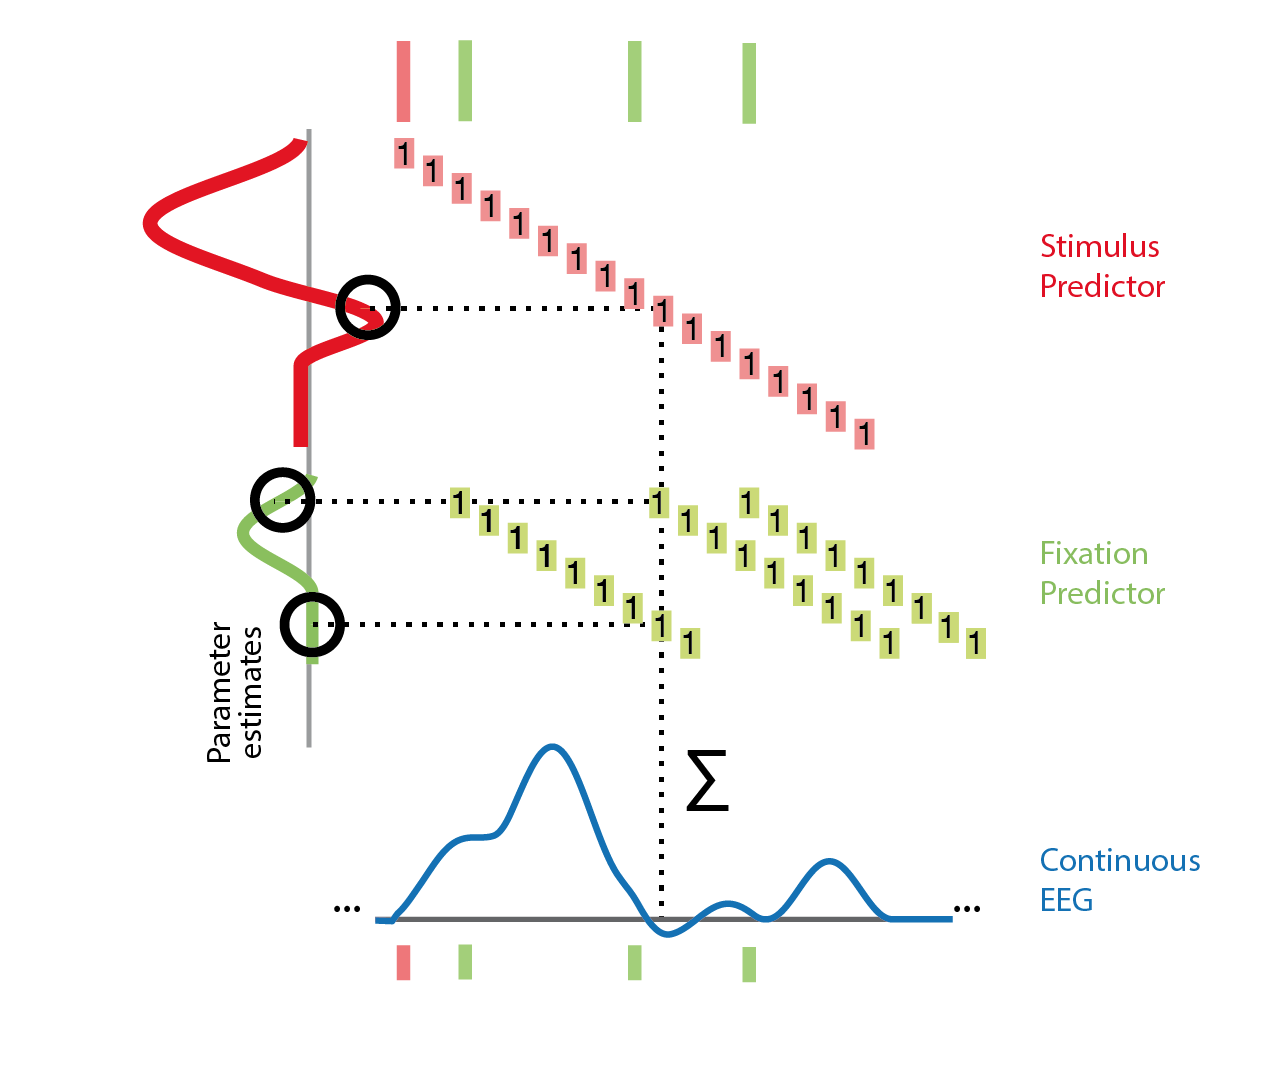
\includegraphics[width=0.5\textwidth]{chapters/01_introduccion/images/esquema_deconvolucion.png}
    \caption{Esquema del método de deconvolución lineal aplicado al EEG continuo. 
    La señal continua (azul) se modela como la suma ponderada de dos predictores 
    temporalmente expandidos: uno para los eventos de estímulo (rojo) y otro para 
    las fijaciones oculares (verde). Los parámetros estimados (izquierda) 
    representan la respuesta neural independiente asociada a cada tipo de evento, 
    es decir, la Temporal Response Function (TRF). Adaptado de \citet{ehinger2019}.}
    \label{fig:deconvolucion}
\end{figure}

Este marco de deconvolución lineal fue aplicado sobre el dataset HSEM por \citep{care2025}, quienes desarrollaron un modelo de TRFs por regresión regularizada para estudiar los correlatos neurales de la búsqueda híbrida. Dicho modelo incorpora predictores definidos a nivel de fijación y sacada y logra recuperar componentes neurales ya documentados en la literatura. Este resultado valida al framework de TRFs como una herramienta apropiada para vincular variables de interés con la señal EEG registrada durante la tarea, y constituye el punto de partida metodológico sobre el cual se apoya la presente tesis.

\subsubsection{Interpretación de las TRFs: regiones cerebrales y componentes de referencia}

Las TRFs estimadas por el modelo producen patrones de actividad
con una estructura espacial y temporal específica: actividad neuronal
que ocurre a latencias determinadas y que se concentra en
regiones particulares del cuero cabelludo. Para poder interpretar estos patrones más adelante, se introducen a continuación los conceptos básicos de neurociencia necesarios: la organización espacial de los electrodos EEG y los componentes neurales de referencia que se retomarán a lo largo de esta tesis.

La señal EEG se registra simultáneamente en múltiples electrodos
distribuidos sobre el cuero cabelludo. Esta distribución espacial permite localizar aproximadamente
qué región cortical genera cada respuesta: los electrodos frontales (ubicados en la parte delantera 
de la cabeza) reflejan procesos cognitivos de alto nivel como
planificación, control atencional y memoria de trabajo;
los electrodos parietales (ubicados en la parte 
trasera) capturan procesos de atención espacial; los electrodos occipitales (ubicados 
en la parte de atrás de la cabeza) capturan principalmente actividad 
de la corteza visual primaria, reflejando el procesamiento visual 
temprano ante cada fijación.


\begin{figure}[H]
    \centering
    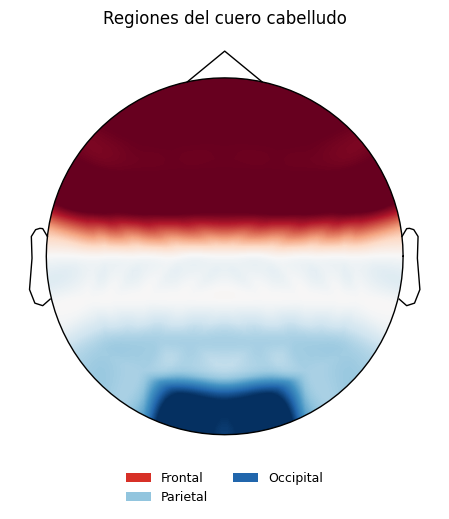
\includegraphics[width=0.3\textwidth]{chapters/02_materiales/images/cabecita_regiones.png}
    \caption{Distribución de las regiones del cuero cabelludo según 
su ubicación anatómica.}
    \label{fig:regiones_corteza}
\end{figure}


La respuesta neural ante un evento puede caracterizarse a través de
\textit{componentes}: patrones de activación de la señal EEG que
ocurren a latencias específicas tras el onset del evento y que están
bien establecidos en la literatura de neurociencia cognitiva. Por
convención, los componentes se nombran según la polaridad de la
activación (positiva (P) o negativa (N)) y su latencia aproximada
en milisegundos. Por ejemplo, el P100 es una activación positiva
que ocurre alrededor de los 100 ms; el N200, una activación negativa
alrededor de los 200 ms.

El \textbf{compontente P100} es un componente positivo temprano
que ocurre entre los 80 y 130 ms tras la presentación de un
estímulo visual, con distribución sobre electrodos occipitales
laterales. Refleja el procesamiento visual temprano ante la llegada de nueva información visual. El P100 puede ser modulado por la atención: su amplitud aumenta cuando el estímulo aparece en una región del
campo visual que el sujeto estaba atendiendo.

El \textbf{componente P300} es un componente positivo tardío que ocurre entre los
250 y 500 ms tras el onset de un estímulo, con pico típico
alrededor de los 300 ms y distribución máxima sobre electrodos
parietales. A diferencia del P100, su ocurrencia no depende de las características físicas del
estímulo sino de la relevancia que ese estímulo tiene para
la tarea en curso. En particular, el P300 se asocia a procesos
de evaluación y categorización del estímulo.

%\pendiente{En caso de aparecer nuevos componentes en el análisis de los resultados de TFCE (en sección resultados), serán agregados y explicados en esta}